% !TEX root = ./main.tex
\documentclass[a4paper]{article}
% Course language: use [english] or [german].
\usepackage[german]{ajnotes}
\title{\textbf{Betriebwirtschaftslehre — Finanzplan}}
\begin{document}
    \maketitle
    % Attach the given problem sheet: drop it in this folder as sheet.pdf and
    % un-comment the next line (pdfpages is already loaded by the preamble).
    % \includepdf[pages=-]{sheet.pdf}
    \textit{siehe}\url{https://lms.uzh.ch/auth/RepositoryEntry/17910989063/CourseNode/82289122624129}
    \section{Finanzplan}
    Beinhaltet:
    \begin{itemize}
        \item Erfolgsrechnung
        \item Angaben des Geschäftsgangs mind. für künftige 5 Jahre (Break-Even erwünscht)
        \item 1. Jahr in Quartale unterteilt, andere als ganze Jahre
        \item Kennzahlen und Annahmen
    \end{itemize}

    \subsection{Elemente}

\begin{enumerate}
    \item Erfolgsrechnung (über Zeitraum) \footnote{siehe Financial Accounting} 
    \begin{itemize}
        \item Bruttogewinn (Warenertrag - Warenaufwand)
        \item Betriebsgewinn EBIT\footnote{Earnings Before Interest and Taxes (EBITDA inkludiert Amortisation)}
        \begin{itemize}
            \item  Ertrag - (Aufwendungen ohne Finanzaufwand und -ertrag,
ohne Ertragssteuern, ohne neutraler Aufwand und Ertrag).
        \end{itemize}
        \item Reingewinn (Alle Erträge - alle Aufwände)
    \end{itemize}
    \item Bilanz (über Zeitpunkte) \footnote{siehe Financial Accounting}
    \item Cashflow-Rechnung 
    \begin{itemize}
        \item Auskunft über die Veränderung der flüssigen Geldmittel (wird )
    \end{itemize} 
\end{enumerate}

\subsubsection{Erfolgsrechnung Prognostizieren}

    \subsection{Finanzierungsquellen}
    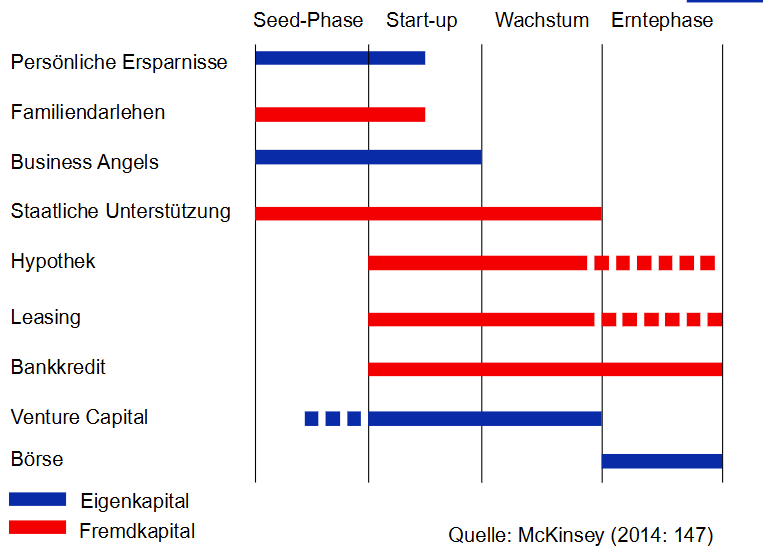
\includegraphics[width=\textwidth,height=0.7\textheight,keepaspectratio]{figures/Finanzierungsquelle.png}
\footnote{\textit{3. Business Angels} kleine Investoren (nicht zuverlässig), \textit{8. Venture Capital} verbunden mit Verlust von Eigentümerrechte, da Venture Capitalists die Führung übernehmen}
    \subsection{Bilanz: Vorgehen}
    \begin{itemize}
        \item Aktiven ermitteln (Umlaufvermögen)
        \begin{itemize}
            \item Kundenforderungen (Debitoren)
            \begin{itemize}
                \item Debitorenbetrag = Umsatz/360 Tage * Zahlungsziel in Tage
            \end{itemize}
            \item Vorräte (Zwischen Warenein- und -ausgang)
            \begin{itemize}
                \item Lagerbestand = (Umsatz / 360 ) * Periode Ein und Ausgang
            \end{itemize}
        \end{itemize}
        \item Aktiven ermitteln (Anlagevermögen)
        \begin{itemize}
            \item Sachanlagen (Maschinen, Immobilien, Fahrzeuge, Mobilien)
            \item Immaterielle Verm.gegenstände (Patente, Lizenzen)
        \end{itemize}
        \item Passiven ermitteln
        \begin{itemize}
            \item FremdKapital
            \begin{itemize}
                \item Kreditorenbetrag  = Verbindlichkeiten / 360 Tagge * Zahlungsziel in Tage
            \end{itemize}
            \item Eigenkapital 
            \begin{itemize}
                \item Kapitalreserven
            \end{itemize}
        \end{itemize}
    \end{itemize}

    \subsection{Cashflow Rechnung}
    \begin{definition}
        [Cashflow] Nettogeldzufluss in einer Zeitperiode
    \end{definition}
    \begin{definition}
        [Break-Even] für Startups: Zeitpunkt ab dem positive Cashflows erzielt werden (bedeutet nicht unbedingt Gewinne). Generell: Gewinnschwelle wurde überschritten.
    \end{definition}
    \begin{definition}
        [Payback-Periode] Zeitraum, worin kumulierte negative Cashflows durch positive kompensiert werden.
    \end{definition}
    \subsubsection{Ziel}
    Die Sicherstellung ausreichender Liquidität oder flüssigen Mittel

\end{document}
